% A simple graph with straight and bend arrows and loops
% Stefan Kottwitz
\documentclass{standalone}
\usepackage{tikz}
\usetikzlibrary{arrows}
\begin{document}
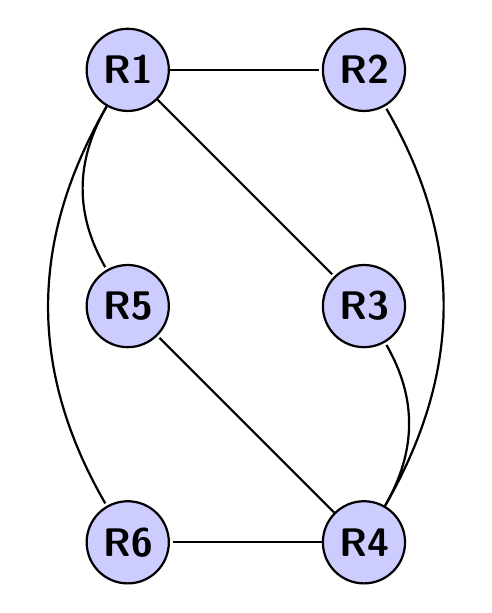
\begin{tikzpicture}[-,>=stealth',shorten >=1pt,auto,node distance=3cm,
  thick,main node/.style={circle,fill=blue!20,draw,font=\sffamily\Large\bfseries}]

  \node[main node] (1) {R1};
  \node[main node] (5) [below of=1] {R5};
  \node[main node] (6) [below of=5] {R6};
  \node[main node] (2) [right of=1] {R2};
  \node[main node] (3) [right of=5] {R3}; 
  \node[main node] (4) [right of=6] {R4};

  \path[every node/.style={font=\sffamily\small}]
    (1) edge node [left] {} (2)
        edge [right] node[left] {} (3)
        edge [bend right] node [left] {} (5)
        edge [bend right] node [left] {} (6)
    (4) edge node [left] {} (5)
        edge [right] node[left] {} (6)
        edge [bend right] node [left] {} (2)
        edge [bend right] node [left] {} (3);
\end{tikzpicture}
\end{document}